\chapter{Previous Research in the Field of Fan Fiction}\label{ch:rw}

% Related Work intro
Fan fiction is an extraordinary resource for a huge variety of freely available texts by as many authors.
Especially in the field of natural language processing (NLP), fan fiction is a great source of material, which many publications take advantage of.


\section{History of German Fan Fiction}\label{sec:history-of-german-fan-fiction}

Since this paper's research is about German fan fiction, it is worthwhile to look at it in terms of its history.
\citet{Cuntz-Leng2015AGermany} state in their ``A Brief history of fan fiction in Germany'' that many fan activities, objects and phenomena in Germany are unique to German culture.
In the early 19th century Karl-May (1842-1912) was (and still is) one of the most widely read, translated and adapted writers~\citep{Petzel2002DasAbenteuer-Mythos}, and the closest thing to a pop-cultural phenomenon.
The growing fan base led to a growth of the German fan fiction community in general, but was abruptly halted by two world wars and the repressive politics of National Socialism.
According to \citet{Odin2008TownsIdentity}, Germans are still struggling with this trauma and loss of identity as of today.
The introduction of the internet and the success of anime and manga~\citep{Malone2010FromEconomically} are said to have been responsible for the resurgence around the year 2000 when with \emph{Animexx}\footnote{https://www.animexx.de/fanfiction/} and \emph{FanFiktion.de}\footnote{https://www.fanfiktion.de/} two fan fiction platforms were founded.
While there were relatively few stories from the genre of anime and manga on Anglo-American fan fiction platforms like \emph{FanFiction.Net}\footnote{https://www.fanfiction.net/} ($25.3\%$) and \emph{Archive of Our Own}\footnote{https://archiveofourown.org/} ($12\%$), there were significantly more on \emph{FanFiktion.de} ($29\%$) and \emph{Animexx} ($49.5\%$), which only reinforces the importance of this genre for German fan fiction culture.
\begin{table}[ht]
    \centering
    \begin{tabular}{lrr}
        \toprule
        \textbf{Fandom} & \textbf{FanFiktion.de} & \textbf{Archive Of Our Own} \\
        \midrule
        Harry Potter    & 36,877 (12.2\%)        & 69,072 (4.8\%)              \\
        Naruto          & 26,404 (8.7\%)         & 9,987 (0.7\%)               \\
        Twilight        & 13,954 (4.6\%)         & 4,397 (0.3\%)               \\
        One Piece       & 8,781 (2.9\%)          & 3,175 (0.2\%)               \\
        One Direction   & 6,308 (2.1\%)          & 33,217 (2.3\%)              \\
        Yu-Gi-Oh!       & 4,522 (1.5\%)          & 2,339 (0.16\%)              \\
        Tokio Hotel     & 4,453 (1.46\%)         & 725 (0.05\%)                \\
        Supernatural    & 3,449 (1.14\%)         & 91,848 (6.3\%)              \\
        Sherlock Holmes & 2,867 (1\%)            & 72,637 (5\%)                \\
        The Avengers    & 1,074 (0.35\%)         & 53,888 (3.7\%)              \\
        Doctor Who      & 677 (0.2\%)            & 36,896 (2.5\%)              \\
        \midrule
        Total           & 303,316                & 1,452,704                   \\
        \bottomrule
    \end{tabular}
    \caption[Top 7 fandoms on \emph{FanFiktion.de} and top 5 on \emph{Archive of Our Own}.]{Top 7 fandoms on \emph{FanFiktion.de} and top 5 on \emph{Archive of Our Own}.
    Adapted from \citet[Table~1]{Cuntz-Leng2015AGermany}.}
    \label{tab:cuntz_2015_german_english_ff_comparison}
\end{table}
Table~\ref{tab:cuntz_2015_german_english_ff_comparison} from Cuntz-Leng and Mentzinger shows that German fan fiction was much less diverse than Anglo-American was.
The \emph{Harry Potter}, \emph{Naruto} and \emph{Twilight} fandoms on FF.de accounted for a very large proportion of German fanfiction in 2015, with over 25 percent of all published stories.
Because each fan fiction community differs in its ``sets of rules, the socialization and education of their members, and the popularity of certain characters, pairings, tropes, or genres'', Cuntz-Leng and Mentzinger contend that generalizing assumptions about fan fiction communities is highly questionable.
They also assumed that German fan fiction writers and readers are more likely to migrate to English-speaking areas of fan culture with their greater variety, larger readership, and less strict youth-protection regulations.

Just as important as the historical and cultural background of fan fiction is analyzing who writes fan fiction.


\section{Analyzing the Authorship and Readership of Fan Fiction}\label{sec:analyzing-the-authorship-and-readership-of-fan-fiction}

Since this paper intends to analyze gender roles, and we assume that they are directly dependent on the author and the reader, it is of particularly high importance to find out how they define themselves.

In the media industry men are observed as the dominating gender in divisions like television shows, news coverage, social media like, like \emph{Twitter}\footnote{https://twitter.com} conversations, and text authors in general~\citep{Milli2016BeyondFanfiction, Bergstrom2012WhatsIt, Bretthauer2007AMusic, Jia2015MeasuringImages, Garcia2014GenderMedia}.
The question now arises as to whether differences can be identified in the area of fan fiction.

\citet{Duggan2020WhoAO3} provides a detailed analysis of people writing \emph{Harry Potter} fan fiction on the online fan fiction repository \emph{Archive Of Our Own} (\emph{AO3}).
Target of research were the contents of almost 2,000 story paratexts as well as their authors user profiles regarding age respectively life stage, gender, location and sexuality.
This wide-scale qualitative study is based on the assumption that fan fiction is no longer the domain of female, white, straight, middle-class, adult and Anglophone people~\citep{Busse2017ACultures, HelleksonBusse2006, Scott2013TextualScott, Lothian2007YearningSpace, Stanfill2011DoingFandom}.
This is due to the fact that fan fiction has become more mainstream~\cite[74]{Barnes2015FanfictionFiction} and more accessible to ``all fans despite their ages, financial means, ethnicities, nationalities, locations, linguistic knowledge, sexualities and genders''~\citep{Duggan2022Worlds...ofFiction}.
Duggan categorizes genders in female, male, trans, genderqueer respectively genderfluid (transgender), non-binary and genderless.
For being able to make statements regarding the text authors gender the pronouns used in story paratexts and profiles were examined (see Table~\ref{tab:duggan_2020_pronouns}).
Despite the fact that the majority of fans on AO3 did not provide any extractable demographic information in their notes, the paper comes to the conclusion that ``gender identity in the \emph{Harry Potter} fandom is much more diverse than previously acknowledged'' based on the data that could be obtained.
While Table~\ref{tab:duggan_2020_gender} shows that 50.39\% stated themselves to be females, 74.02\% preferred she/her(s) pronouns (see Table~\ref{tab:duggan_2020_pronouns}) why it can be inferred that the actually number lies somewhere between those values.
\begin{table}[ht]
    \centering
    \begin{tabular}{lrr}
        \toprule
        \textbf{Gender} & \textbf{Frequency} & \textbf{Percentage} \\
        \midrule
        Female          & 64                 & 50.39\%             \\
        Non-binary      & 27                 & 21.26\%             \\
        Male            & 17                 & 13.39\%             \\
        Transgender     & 14                 & 11.02\%             \\
        Genderless      & 5                  & 3.94\%              \\
        \bottomrule
    \end{tabular}
    \caption[Gender distribution in \emph{AO3} paratexts.]{Gender distribution in \emph{AO3} paratexts.
    Adapted from \citet[Table~1]{Duggan2020WhoAO3}.}
    \label{tab:duggan_2020_gender}
\end{table}
\begin{table}[ht]
    \centering
    \begin{tabular}{lrr}
        \toprule
        \textbf{Preferred pronoun(s)} & \textbf{Frequency} & \textbf{Percentage} \\
        \midrule
        She                           & 94                 & 74.02\%             \\
        He                            & 17                 & 13.39\%             \\
        They                          & 6                  & 4.72\%              \\
        She/They                      & 4                  & 3.15\%              \\
        She/He/They                   & 2                  & 1.57\%              \\
        ``Pronounless''               & 2                  & 1.57\%              \\
        He/They                       & 1                  & 0.79\%              \\
        She/He                        & 1                  & 0.79\%              \\
        \bottomrule
    \end{tabular}
    \caption[Preferred pronoun distribution in \emph{AO3} paratexts.]{Preferred pronoun distribution in \emph{AO3} paratexts.
    Adapted from \citet[Table~2]{Duggan2020WhoAO3}.}
    \label{tab:duggan_2020_pronouns}
\end{table}
With 36.22\% non-cis individuals like genderless, non-binary and transgender outline a much larger group than previously anticipated.
Though one should assume that heteronormativity is regarded as default and is therefore not being particularly emphasized by the authors.
Lastly only 13.39\% reported themselves to be male.
There were no distinctions made between various types of genres and fandoms and rather viewed from a more general perspective.

From this it can be deduced that female individuals make up the larger proportion of readers and authors of fan fiction compared to male individuals.
Assuming that the \emph{Harry Potter} fandom can be generalized and mapped to the entire sector of fiction.


\section{Stereotypes and Gender Bias in Fan Fiction}\label{sec:stereotypes-and-gender-bias-in-fan-fiction}
Based on the assumption that the majority of fan fiction is written by women, is it possible to draw conclusions about differences in stereotypes and gender bias?

In analyzing films, books and music lyrics, women tend to be portrayed as younger, domestic, rather emotional than rational, and with a greater focus on beauty than on their intellect~\citep{Towbin2004ImagesAnimatedFilms, Gooden2001Gender19951999}.
In comparison, men are portrayed as physically stronger and more active, more violent, more economically successful, less in control of their sexuality, and emotionally cold~\citep{Emons2010HeTelevision, Bretthauer2007AMusic, Lauzen2008ConstructingTelevision, Soulliere2006WrestlingWWE}.

% Fast et al. 2016: Shirtless and dangerous: Quantifying linguistic signals of gender bias in an online fiction writing community
In a comprehensive study on a dataset of more than 1.8 billion words from the \emph{Wattpad}\footnote{https://www.wattpad.com} writing community \citet{Fast2016ShirtlessCommunity} investigated gender bias and stereotypical questions.
High-level gender statistics provided by \emph{Wattpad} on request could not confirm \citet{Duggan2020WhoAO3}$'$s thesis regarding an overrepresentation of female authors (male/female ratio was 1.16 for 655,295 stories).
To address the question of how the gender of the characters affects the actions, they examined the verbs that referred to each character.
Both male stereotypes with common verbs like \emph{thrush}, \emph{abuse} or \emph{roar}, and female stereotypes with verbs like \emph{squeal}, \emph{giggle} or \emph{shriek} could be verified with this method.
It was noteworthy, however, that the \emph{angry man} stereotype failed to show up and verbs in this category tended to have darker connotations (like \emph{beat}, \emph{rip} or \emph{snarl}).

\begin{table}[ht]
    \centering
    \begin{tabular}{lrl}
        \toprule
        \textbf{Female} & \textbf{Odds} & \textbf{Sample verbs and adjectives (female odds)}    \\
        \midrule
        weak            & 1.73          & fragile (6.3), faint (3.2), sick (1.8), tired (1.4)   \\
        submissive      & 1.66          & helpless (3.5), shy (2.9), timid (2.8), whimper (1.7) \\
        childish        & 1.54          & squeal (11.1), naive (7.8), giggle (4.9), silly (1.7) \\
        afraid          & 1.46          & shriek (4.8), frightened (2.3), shiver (1.8)          \\
        dependent       & 1.43          & clingy (3.2), vulnerable (2.5), desperate (1.8)       \\
        hysterical      & 1.25          & bitchy (11.4), dramatic (3.2), suicidal (3.1)         \\
        domestic        & 1.16          & cook (2.3), wash (1.8), marry (1.7), clean (1.5)      \\
        emotional       & 1.04          & meanest (7.9), gush (5.1), sob (37), fiery (2.8)      \\
        angry           & 1.05          & bellow (3.1), growl (2.7), curse (1.4), snarl (1.3)   \\
        \bottomrule
    \end{tabular}
    \caption[Dominant female stereotype categories.]{Dominant female stereotype categories. Adapted from \citet[Table2]{Fast2016ShirtlessCommunity}.}
    \label{tab:fast_2016_stereotype_categories_female}
\end{table}

\begin{table}[ht]
    \centering
    \begin{tabular}{lrl}
        \toprule
        \textbf{Male} & \textbf{Odds} & \textbf{Sample verbs and adjectives (male odds)}         \\
        \midrule
        strong        & 2.02          & intense (3.1), smash (2.6), intimidating (2.1)           \\
        arrogant      & 1.30          & cocky (7.1), smirk (2.8), smug (2.6), rude (1.4)         \\
        sexual        & 1.22          & sexiest (3.1), kiss (2.4), hot (2.1), flirt (1.5)        \\
        active        & 1.17          & jog (2.5), lift (2.4), dodge (1.7), spin (1.4)           \\
        dominant      & 1.15          & rich (28), protective (2.7), royal (2.0), command (1.4)  \\
        violent       & 1.10          & abuse (4.4), hurt (2.3), beat (2.0), kill (1.5)          \\
        beautiful     & 1.06          & dreamy (8.14), attractive (4.09), cute (3.3), hot (2.14) \\
        angry         & 1.05          & bellow (3.1), growl (2.7), curse (1.4), snarl (1.3)      \\
        \bottomrule
    \end{tabular}
    \caption[Dominant male stereotype categories.]{Dominant male stereotype categories. Adapted from \citet[Table~2]{Fast2016ShirtlessCommunity}.}
    \label{tab:fast_2016_stereotype_categories_male}
\end{table}

They further investigated which adjectives were used to describe characters and categorized these as well as depicted in~\ref{tab:fast_2016_stereotype_categories_female} and~\ref{tab:fast_2016_stereotype_categories_male}.
In general, stereotypical characteristics were confirmed here as well, but a relatively large number of male characters were described with the rather feminine adjective \emph{beautiful}.
As a third hypothesis, they explored the question of how stereotypes in stories affect their user ratings.
They find that many common stereotypes, such as sexual, arrogant and violent men, have a positive impact on the ratings, while others, such as strong women or domestic men, have a negative impact (see~\ref{tab:fast_2016_stereotype_categories_ratings}).

\begin{table}[ht]
    \centering
    \begin{tabular}{lrlr}
        \toprule
        \textbf{Positive with rating} & \textbf{Coefficient} & \textbf{Negative with rating} & \textbf{Coefficient} \\
        \midrule
        sexual (male)                 & +2.03                & strong (female)               & -0.96                \\
        arrogant (male)               & +1.45                & domestic (male)               & -0.66                \\
        sexual (female)               & +1.24                & afraid (female)               & -0.66                \\
        violence (male)               & +0.92                & weak (male)                   & -0.63                \\
        active (male)                 & +0.90                & domestic (female)             & -0.57                \\
        hysterical (male)             & +0.59                & strong (male)                 & -0.51                \\
        hysterical (female)           & +0.57                & dominant (female)             & -0.44                \\
        anger (male)                  & +0.56                & emotional (female)            & -0.44                \\
        violence (female)             & +0.46                & beautiful (female)            & -0.39                \\
        childish (male)               & +0.42                & weak (female)                 & -0.34                \\
        angry (female)                & +0.20                & dependent (female)            & -0.25                \\
        emotional (male)              & +0.12                & childish (female)             & -0.21                \\
        submissive (female)           & +0.02                & active (female)               & -0.03                \\
        \bottomrule
    \end{tabular}
    \caption[Categories of stereotype with positive respectively negative effects on story ratings in a logistic regression.]{Categories of stereotype with positive respectively negative effects on story ratings in a logistic regression. Adapted from \citet[Table~4]{Fast2016ShirtlessCommunity}.}
    \label{tab:fast_2016_stereotype_categories_ratings}
\end{table}

Finally, they investigated whether female authors stereotyped men in their stories and vice versa.
To this end, they trained a logistic regression model with frequency counts of words captured by their stereotype categories as feature inputs for male and female characters.
The goal here was to predict the authors gender of a story.
However, due to stereotypical features, the author could not be specified by the model and achieved only 53\% accuracy, so the authors concluded that both men and women write indistinguishably stereotypical genders.

% TODO: transition


\section{Possibilities for Natural Language Processing}\label{sec:possibilities-for-nlp}

% Milli & Bamman 2016: Beyond Canonical Texts: A Computational Analysis of Fanfiction
One of the early works focusing on similar aspects of source of material and research topic as this paper is a proceedings paper by \citet{Milli2016BeyondFanfiction}.
In their work they analyzed the possibilities provided by fan fictional texts for NLP, computational social science and the digital humanities in general.
Large-scale literary data as well as a vibrant social network provide a huge opportunity for research in these areas.
A large fan fiction corpus as depicted in Table~\ref{tab:milli_2016_corpus_summary} was collected from \emph{FanFiction.Net} and served as study object.
%\begin{figure}
%    \begin{floatrow}
%        \ffigbox{}{
%            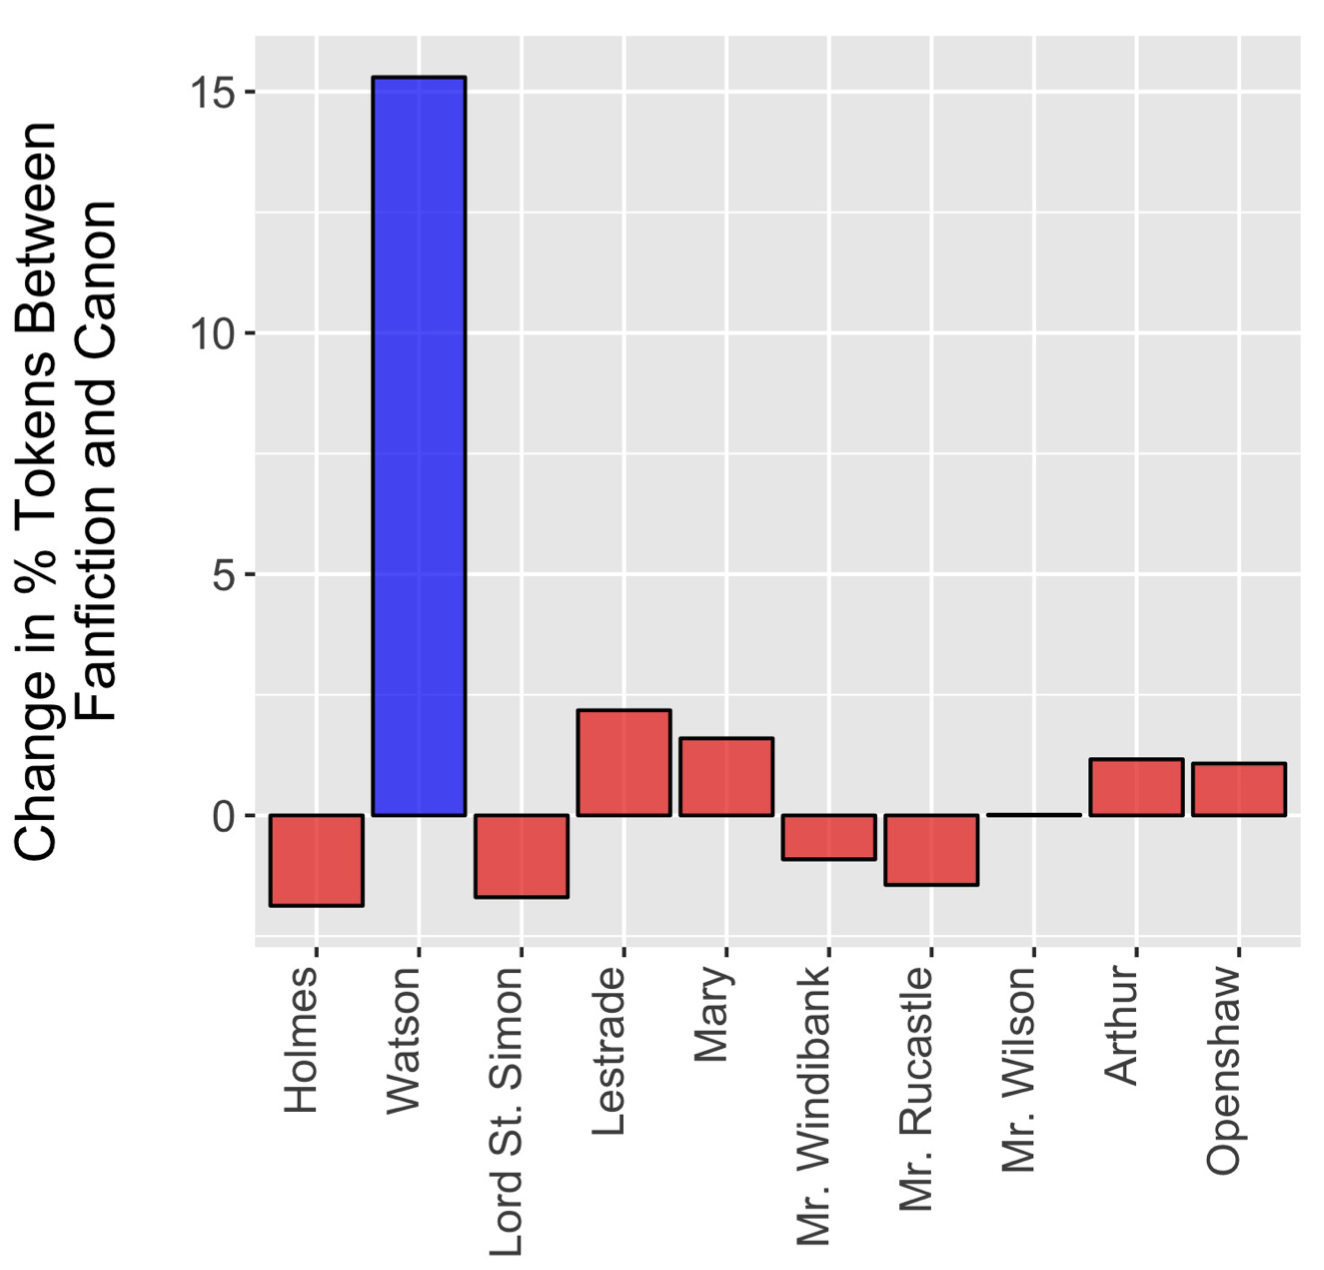
\includegraphics[width=0.5\textwidth]{figures/milli_2016_sherlock_holmes}
%            \caption[Difference in percent character mentions between fan fiction and canon for \emph{Sherlock Holmes}.]{Difference in percent character mentions between fan fiction and canon for \emph{Sherlock Holmes} \citep{Milli2016BeyondFanfiction}.}
%            \label{fig:milli_2016_sherlock_holmes2}
%        }
%        \capbtabbox{
%            \begin{tabular}{lr}
%                \toprule
%                \textbf{Type} & \textbf{Count} \\
%                \midrule
%                Canons        & 9,246          \\
%                Stories       & 5,983,038      \\
%                Tokens        & 55,264,185,653 \\
%                Reviews       & 159,914,877    \\
%                Users         & 2,093,601      \\
%                – Authors     & 1,364,729      \\
%                – Reviewers   & 1,438,721      \\
%                Languages     & 44             \\
%                \bottomrule
%            \end{tabular}
%        }{
%            \caption{A table}
%            \label{tab:table}
%        }
%    \end{floatrow}
%\end{figure}

\begin{table}[ht]
    \centering
    \begin{tabular}{lr}
        \toprule
        \textbf{Type} & \textbf{Count} \\
        \midrule
        Canons        & 9,246          \\
        Stories       & 5,983,038      \\
        Tokens        & 55,264,185,653 \\
        Reviews       & 159,914,877    \\
        Users         & 2,093,601      \\
        – Authors     & 1,364,729      \\
        – Reviewers   & 1,438,721      \\
        Languages     & 44             \\
        \bottomrule
    \end{tabular}
    \caption[Summary of the \emph{FanFiction.Net} corpus.]{Summary of the \emph{FanFiction.Net} corpus.
    Adapted from \citet[p.~2049]{Milli2016BeyondFanfiction}.}
    \label{tab:milli_2016_corpus_summary}
\end{table}
% maybe earlier in my introduction?
They stated that fan fiction with its mainly female authorship~\citep{Duggan2020WhoAO3, Barnes2015FanfictionFiction} deprioritizes the main protagonists, which are mostly male, and consists in return of more and stronger female characters~\citep{Handley2012DistressingFanfiction, Scodari2000CreatingOnline, Leow2011SubvertingFiction, Busse2009InIntroduction}.
For extracting and comparing characters they utilized the Natural Language Processing pipeline \emph{BookNLP}~\citep{Bamman2014ACharacter}.
While freely available canonical texts from \emph{Project Gutenberg}\footnote{https://www.gutenberg.org} serve as object of comparison, Milli \& Bamman can proof their hypothesis regarding deprioritization with a statistical significance of $p < 0.001$ (40.1\% female characters in canonical texts to 42.1\% in fan-written texts).
% TODO: dreprioritization of FEMALE or MAIN CHARACTERS?
\begin{figure}
    \centering
    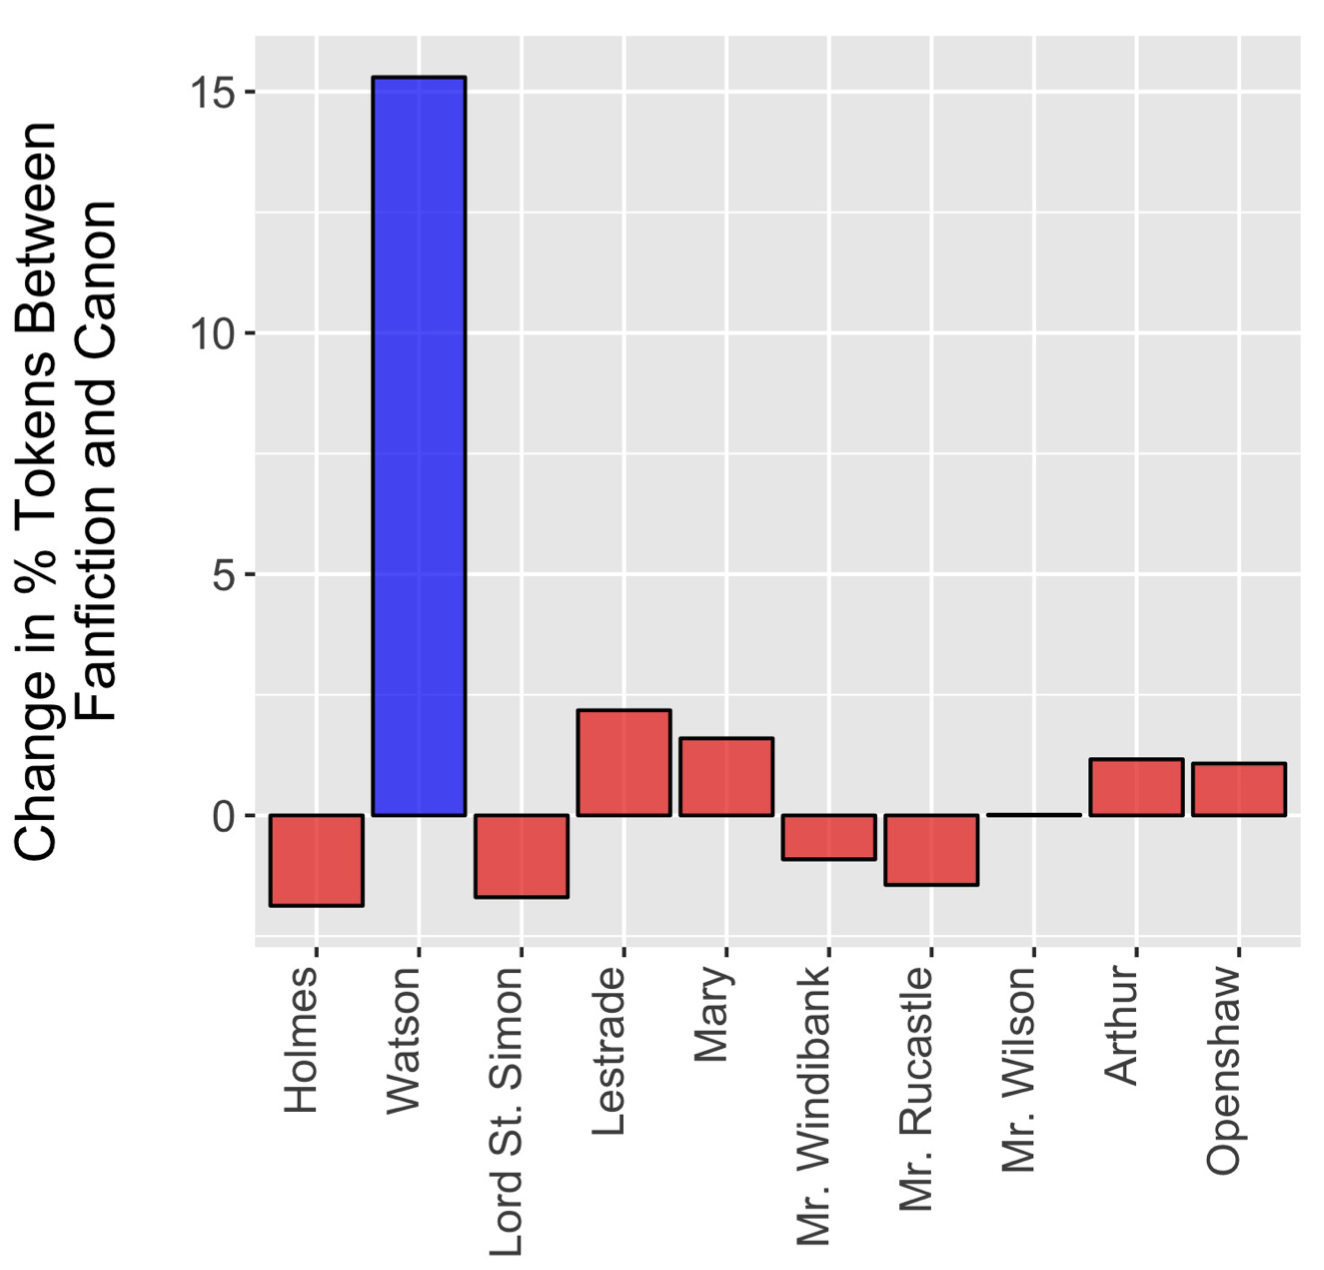
\includegraphics[width=0.5\textwidth]{figures/milli_2016_sherlock_holmes}
    \caption[Difference in percent character mentions between fan fiction and canon for \emph{Sherlock Holmes}.]{Difference in percent character mentions between fan fiction and canon for \emph{Sherlock Holmes}.
    Reprinted from~\cite[p.~2049]{Milli2016BeyondFanfiction}.}
    \label{fig:milli_2016_sherlock_holmes}
\end{figure}

As an example they presented in Figure~\ref{fig:milli_2016_sherlock_holmes} the difference of character appearances in texts about the \emph{Sherlock Holmes} fandom.
A secondary character as in \emph{Watson} receives substantially more mentions in fan fiction than in the canonical text, while the main character (\emph{Sherlock Holmes}) loses them slightly.

Furthermore, they identified that more than half of the fan-authors (52\%) are in return reviewers of other works.
In an exploratory analysis they ran a Latent Dirichlet Allocation model~\citep{Blei2003LatentAllocation} on the review texts and determined that most reviews are about positive encouragement, pleas for updates, requests to the author about the progression of the story and emotional reactions.
For training a sentiment classifier predicting the users reactions in reviews they conducted a study asking the participants to judge the sentiment towards the character expressed in the response (positive, negative, neutral or not applicable).

% Yin et al: Where No One Has Gone Before: A Meta-Dataset of the World's Largest Fanfiction Repository
% > https://dl.acm.org/doi/abs/10.1145/3025453.3025720?casa_token=BjEEdi0q0N4AAAAA:ZtJvcEJtzZy316s25giI4h1i5tR3eFGsBZQ1BxtBOMZ_ypD-WRnrwhc8fnhp0OlMP344boDG-D8W

While there are other works highlighting the possibilities that these large quantities of diversely written texts provide, they pursue other approaches that are impractical or beyond the scope of this research paper.

One of a few popular mentions is \citet{Liu2019DENS:Analysis} who fine-tuned a pre-trained BERT model for a multi-class emotion analysis using texts from previously mentioned \emph{Project Gutenberg} and \emph{Wattpad}, another platform intended for users to read and write stories.

\citet{Muttenthaler2019AuthorshipN-grams} developed and compared three n-gram models to identify authors of fan-fictional texts.
They concluded that their standard n-gram model (2 - 5 gram) performed best and a combination of different text representations best reflects the author's writing style.

The task of predicting upcoming actions from textual descriptions of scenes using \emph{Harry Potter} fan fiction was examined by \citet{Vilares2019HarryLanguage}.
A model based on an LSTM, a recurrent neural network with feedback connections, performed best for frequent actions and extensive scene descriptions, while logistic regression performed well for infrequent actions.

By collecting a million stories and their summaries on \emph{Wattpad}, \citet{Zhang2019GeneratingFiction} identified common components to describe the stories' characters.
The objective of the work was to automatically generate these character summaries using inferring salient attributes.
They developed two models of which one extracted and used attributes from the source story by ranking them, while the other classified abstractly using a list of attributes drawn from the entire corpus of stories which performed better.

\citet{Kleindienst2020InvestigatingSupernatural} took a more specific approach and studied only one fandom, the quite popular TV show \emph{Supernatural} (see also~\ref{tab:schmidt_2021_ao3_corpus}).
In doing so, they examined how the fan fiction community adapted to the source material over the time the show ran using, while using the show's scripts and 7,000 texts from the AO3 platform.
They can confirm the thesis of \citet{Milli2016BeyondFanfiction} concerning the overrepresentation of secondary characters and observed an overwhelming amount of male-male relationships in fan fiction ($91.99\%$; \citet{Tosenberger2008HomosexualityFanfiction, HelleksonBusse2006, Duggan2017RevisingFanfiction}) compared to the source material.

% etwas größer als nur 1 fandom: crossover
Not just one specific fandom, but rather the combination of individual fandoms, the so-called crossovers, were investigated by \citet{Schmidt2022AnalyzingOwn}.
They used a tool named \emph{Gephi}\footnote{https://gephi.org/} for a computational social network analysis (SNA) depicting unique character relationships visually.
They found that original characters are important for crossovers, and that popular fandoms, stories of the same genre (e.g.\ Sci-Fi) and nationality (e.g.\ British as in \emph{Sherlock Holmes} and \emph{James Bond}) are often linked.

These are just a few examples that show the possibilities offered by the analysis and study of fan-fictional texts.


\section{Analyzing German Fan Fiction}\label{sec:german-fan-fiction} % TODO: working title

Because most fan fiction gets published in the english language and though an increasing number of german authors tend to switch to it as well~\citep{Cuntz-Leng2015AGermany}, research focuses primarily on english-written texts.

% Schmidt et al. 2021: Towards the Analysis of Fan Fictions in German Language: Exploration of a Corpus from the Platform Archive of Our Own

\citet{Cuntz-Leng2015AGermany} stated in their paper about the history of german fan fiction that style, content and progression of fan fiction differ on a cultural background.
Which is why \citet{Schmidt2021TowardsOwn} gathered a corpus of 9,640 german writings from the previously mentioned \emph{AO3} platform for analysis.
While metadata and general text statistics like the most frequent words were the subject of the investigation, they identified ``attributes that are very specific and unique to German culture''.
\begin{table}[ht]
    \centering
    \begin{tabular}{lrr}
        \toprule
        \textbf{Fandom} &
        \textbf{Frequency} &
        \textbf{Percentage} \\
        \midrule
        Tatort              & 986   & 10.2\% \\
        Harry Potter        & 800   & 8.3\%  \\
        Supernatural        & 413   & 4.3\%  \\
        Sherlock (TV)       & 405   & 4.2\%  \\
        Original Work       & 349   & 3.6\%  \\
        Football RPF        & 295   & 3.1\%  \\
        Stargate Atlantis   & 220   & 2.3\%  \\
        Stargate SG         & 191   & 2.0\%  \\
        Historical RPF      & 151   & 1.6\%  \\
        Glee                & 141   & 1.5\%  \\
        \midrule
        Rest (1,603 Fandoms) & 5,830 & 58.9\% \\
        \bottomrule
    \end{tabular}
    \caption[Top 10 fandoms of the \emph{AO3} corpus.]{Top 10 fandoms of the \emph{AO3} corpus.
    Adapted from \citet[p.~4]{Schmidt2021TowardsOwn}.}
    \label{tab:schmidt_2021_ao3_corpus}
\end{table}
Next to popular fan fiction fandoms like \emph{Harry Potter} and \emph{Supernatural}, \emph{Tatort}, a german crime television show, real person fan fiction (\emph{RPF}; e.g. \emph{Football}) as well as stories about \emph{Goethe} and \emph{Schiller} (\emph{Historical RPF}) were often used as source material as seen in~\ref{tab:schmidt_2021_ao3_corpus}.
The assumption that \emph{Anime} is strongly related to the rise of fan fiction in Germany~\citep{Cuntz-Leng2015AGermany} could not be reflected in the AO3 corpus consisting only of 97 stories.
It was also noticeable that all-male romances (56\%), male characters in general (see also~\ref{sec:possibilities-for-nlp} respectively \citet{Kleindienst2020InvestigatingSupernatural}), and an excess of stories of an erotic nature dominated the corpus.
The fascination that fan fiction has with same-sex relationships has already been identified and analyzed in the humanities by \citet{HelleksonBusse2006}, \citet{Tosenberger2008HomosexualityFanfiction} and \citet{Duggan2017RevisingFanfiction}.
Furthermore, after analyzing the most frequently occurring words in the corpus, they were able to determine that they are strikingly often words that describe physical attributes.

% TODO: transition to the main part

% NOT USED:
% Hellekson & Busse: Fan Fiction and Fan Communities in the Age of the Internet: New Essays.
% > https://books.google.de/books?hl=de&lr=&id=11ODBAAAQBAJ&oi=fnd&pg=PP1&dq=Fan+Fiction+and+Fan+Communities+in+the+Age+of+the+Internet:+New+Essays.&ots=3AViPB5RG6&sig=RrWdSLLLWFStJeF7aNJQv3owuhQ#v=onepage&q=Fan%20Fiction%20and%20Fan%20Communities%20in%20the%20Age%20of%20the%20Internet%3A%20New%20Essays.&f=false
% highlight the striking dominance of slash fan fiction (stories focused on male-male romantic and erotic relationships) in the fan fiction community
